\chapter{Аналитический раздел}\label{sec:analyth}

В данном разделе будет проведен анализ существующих решений, формализованы требования к приложению и определены пользователи системы.

%\section{Постановка задачи}
%
%Необходимо разработать приложение, позволяющее спортсменам по фехтованию ориентироваться в календаре турниров и отслеживать ближайшие соревнования.

\section{Анализ существующих решений}

В таблице \ref{tab-exists} представлено сравнение существующих решений по ряду критериев. 

В таблице \ref{tab-exists} используются следующие сокращения:

\begin{itemize}
	\item ФФР --- официальный портал федерации фехтования России \cite{FIE};
	\item En Garde --- официальный портал одного из крупнейших клубов фехтования г. Москвы \cite{EnGarde}.
\end{itemize}

\begin{table}[H]
	\centering
	\caption{Анализ существующих решений}
	\renewcommand{\arraystretch}{1.8}
	\resizebox{\textwidth}{!}{
		\begin{tabular}{|c|c|c|}
			\hline
			Критерии/существующие решения & ФФР & En Garde \\ \hline
			Предоставление информации о каждом спортсмене & + & - \\ \hline
			Календарь соревнований & + & + \\ \hline
			Общие результаты соревнований & + & + \\ \hline
			Новости спорта & + & + \\ \hline
			Результаты соревнований конкретного спортсмена & + & - \\ \hline
			Авторизация & - & - \\ \hline
			Возможность самостоятельно подавать заявку на турнир & - & - \\ \hline
		\end{tabular}
	}
\label{tab-exists}
\end{table}

Рассмотренные решения являются информационными порталами, которые не предоставляют возможность авторизации и, как следствие, самостоятельной подачи заявки на турнир. Данная возможность станет ключевой отличительной чертой разрабатываемого приложения.

\section{Требования к приложению}

На основе проведенного выше анализа существующих решений можно выдвинуть следующие требования к приложению:

\begin{itemize}
	\item регистрации и авторизации пользователей;
	\item подачи заявки на выбранный турнир;
	\item просмотра всех соревнований;
	\item добавления нового турнира;
\end{itemize}

\section{Пользователи системы}

В таблице \ref{tab:users-type} представлены типы пользователей и соответствующий им функционал.

\begin{table}[H]
	\centering
	\caption{Типы пользователей}
	\renewcommand{\arraystretch}{1.8}
	\resizebox{\textwidth}{!}{
\begin{tabular}{|p{0.3\textwidth}|p{0.6\textwidth}| }
	\hline
	Тип пользователя & Функционал \\
	\hline
%	\hline 
	Неавторизованный  & Регистрация, авторизация, просмотр календаря соревнований и общей информации о всех турнирах \\ \hline
	Авторизованный & Просмотр общей информации о турнирах, возможность подачи заявки на интересующие соревнования \\ \hline
	Администратор & Просмотр общей информации о турнирах, \newline Изменение различной информации о соревнованиях и их участниках. \newline Добавление нового турнира \newline Изменение ролей пользователей \\
	\hline
\end{tabular}
}
\label{tab:users-type}
\end{table}

На рисунке \ref{ris:usecase} представлена диаграмма использования приложения.

\begin{figure}[H]
	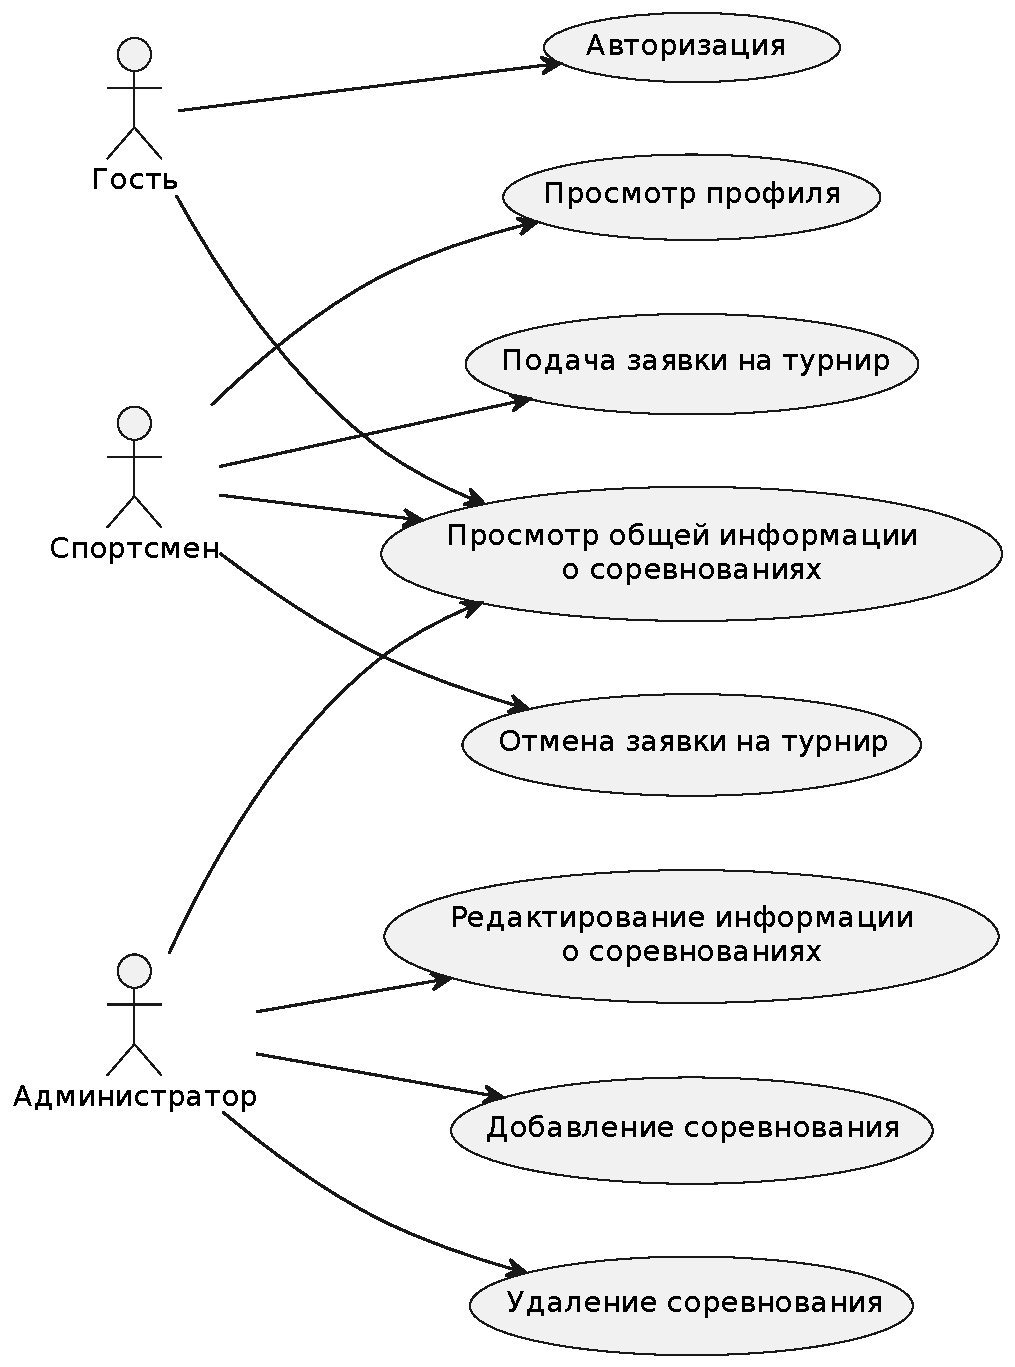
\includegraphics[width=0.6\columnwidth]{assets/out/usecase/usecase.pdf}
	\centering
	\caption{Use-case диаграмма}
	\label{ris:usecase}
\end{figure}

\section{Формализация данных}

База данных состоит из следующих таблиц:

\begin{itemize}
	\item таблица аккаунта;
	\item таблица соревнований;
	\item таблица проведенных боев;
	\item таблица информации о спортсмене;
\end{itemize}

На рисунке \ref{ris:er} представлена ER-диаграмма приложения.

\begin{figure}[H]
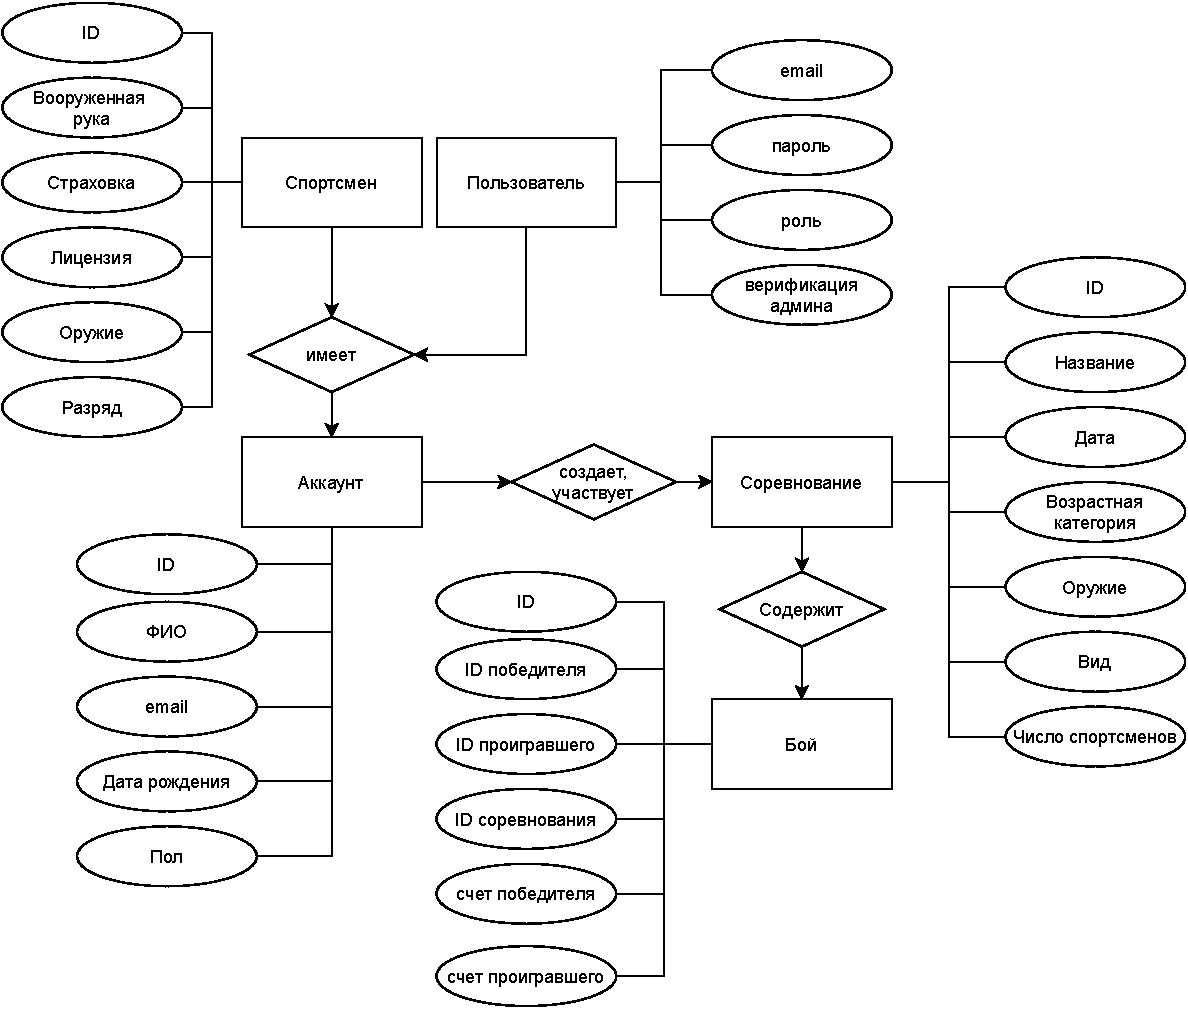
\includegraphics[width=1\columnwidth]{assets/er.drawio.pdf}
\centering
\caption{ER-диаграмма в нотации Чена}
\label{ris:er}
\end{figure}

\section{Модели данных}

Модель данных --- это систематизация разнообразной информации и отражение ее свойств по содержанию, структуре, объему, связям, динамике с учетом удовлетворения информационных потребностей всех категорий пользователей \cite{models}.

\begin{enumerate}
	\item Дореляционные модели данных:
	\begin{itemize}
		\item Иерархическая модель --- структура, в которой объекты делятся на родителей и потомков. При этом у каждого потомка может быть не более одного родителя. Графическим представлением является древовидная структура.
		
		Примеры: организация файловых систем; DNS и LDAP-соединения;
		
		\item Сетевая модель --- структура, в которой каждый элемент может быть связан с любым другим элементом. Сетевая база данных состоит из наборов записей, которые связаны между собой так, что записи могут содержать явные ссылки на другие наборы записей, образуя тем самым сеть \cite{models}
		
		Пример: IDMS --- специализированная СУБД для мейнфреймов.
	\end{itemize}
	
	\item Реляционная модель представляет собой совокупность данных, состоящую из набора таблиц. При такой организации данных отсутствует какая-либо иерархия между элементами \cite{rel}.
	
	Примеры: MySQL, MariaDB, SQLite и др. 
	
	\item Постреляционная модель данных является расширением реляционной модели. Она снимает ограничение неделимости данных, допуская многозначные поля, значения которых состоят из подзначений, и набор значений воспринимается как самостоятельная таблица, встроенная в главную таблицу \cite{post}.
	
	Примеры:  UniVerse (Vmark Software), Cache’ (Intersystems), Postgres
	
	\item Модель <<ключ-значение>> --- модель, более известная как словарь или хеш-таблица, которая хранит коллекции объектов или записей. Такая модель рассматривает данные как отдельную коллекцию, каждая запись в которой может иметь множество различных полей \cite{key-value}.
	
	Примеры: Amazon, DynamoDB, Redis, Riak, LevelDB, различные хранилища кэша – например, Memcached и пр.
	
	\item Многомерная модель данных --- модель данных, информация в которой представляется в виде многомерных массивов, называемых гиперкубами. В одной базе данных, построенной на многомерной модели, может храниться множество таких кубов, на основе которого можно проводить совместный анализ показателей \cite{post}.
	
	Примеры: Essbase (фирма Arbor Software), Media Multi-matrix (фирма Speedware) и др.
	
	\item Объектно-ориентированная модель данных --- это структура, которую можно изобразить графически в виде дерева, узлами которого являются объекты. Между записями базы данных и функциями их обработки устанавливаются связи с помощью механизмов, подобных тем, которые имеются в объектно-ориентированных языках программирования \cite{post}.
	
%	\item Графовые базы данных --- базы данных, которые используют графовые структуры для семантических запросов с узлами, ребрами и свойствами для представления и хранения данных. Графовая модель --- это разновидность сетевой модели, реализованной в виде графа, однако сетевая модель работает на более низком уровне абстракции \cite{Angles2008} и не имеет легкого обхода по цепочке ребер \cite{Silberschatz2010}.
%	
%	Примеры: Neo4J, JanusGraph, Dgraph, OrientDB.
	
\end{enumerate}

\section{Вывод}

В данном разделе был проведен анализ существующих решений, на основе которого были выдвинуты требования к разрабатываемому приложению, выделены ролевые модели системы, формализованы хранимые данные, а также описаны существующие типы баз данных, вывод о недостатках и преимуществах которых представлен в таблице \ref{tab:class}.

\begin{table}[H]
	\centering
	\caption{Преимущества и недостатки различных моделей данных}
	\renewcommand{\arraystretch}{1.8}
	\resizebox{\textwidth}{!}{
		\begin{tabular}{|p{0.3\textwidth}|p{0.4\textwidth}| p{0.4\textwidth}|}
			\hline
			Название & Преимущества & Недостатки \\
			\hline
			Дореляционные (иерархическая, сетевая) & Возможна эффективная реализация по показателям затрат памяти и оперативности  & Не предполагает связи <<многие ко многим>>, сложность и жесткость схемы базы и, как следствие, сложность реорганизации \\ \hline
			Реляционные & Возможно минимизировать объем базы данных, повысить целостность системы и отказоустойчивость, упростить масштабирование & Жесткая структура сведений об объектах, сложность реорганизации \\ \hline
			Постреляционная & Возможность представления совокупности связанных реляционных таблиц в виде одной постреляционной таблицы & Сложность решения проблемы поддержания целостности и непротиворечивости данных\\ \hline
			<<Ключ-значение>> & Возможно хранение и обработка разных по типу и содержанию данных, высокая скорость доступа к данным за счет адресного хранения, легкое масштабирование & На разработчика клиентского приложения ложится ответственность за контроль валидности данных, сложность решения проблемы поддержания целостности и непротиворечивости данных\\ \hline
			Многомерная & Удобство и эффективность анализа больших объемов данных, имеющих временную связь, а также быстрота реализации сложных, нерегламентированных запросов & Громоздкость при использовании для стандартных задач, не эффективное использование памяти, т\,к в данной модели резервируется место для всех значений, даже ели некоторые из них будут отсутствовать \\ \hline
			Объектно-ориентированная & Возможность отображения информации о сложных взаимосвязях объектов и идентификации отдельных записей в базе с определением функций их обработки & Сложность понимания сути модели и низкая скорость выполнения запросов\\ \hline
%			Графовые & Возможность организации сложных взаимосвязей, использование более естественного подхода к данным, легкость расширения и изменения & Отсутствие гарантии целостности данных, отсутствие возможностей атомарности транзакции и согласования данных при одновременном выполнении транзакций на уровне БД \\ \hline			
		\end{tabular}
	}
	\label{tab:class}
\end{table}


%
%\section{Постановка задачи}
%
%Необходимо разработать программу для отображения информации о соревнованиях и их результатах, а также предоставить каждому спортсмену и его тренеру индивидуальную информацию о результатах прошедших турниров и предстоящих возможных соревнованиях.
%
%\section{Анализ существующих решений}
%
%В таблице \ref{tab-exists} представлено сравнение существующих решений по ряду критериев. 
%
%В таблице \ref{tab-exists} используются следующие сокращения:
%
%\begin{itemize}
%	\item ФФР --- официальный портал федерации фехтования России;
%	\item En Garde --- официальный портал одного из крупнейших клубов фехтования г. Москвы.
%\end{itemize}
%
%\begin{table}[H]
%	\centering
%	\caption{Анализ существующих решений}
%	\renewcommand{\arraystretch}{1.8}
%	\resizebox{\textwidth}{!}{
%		\begin{tabular}{|c|c|c|}
%			\hline
%			Критерии/существующие решения & ФФР & En Garde \\ \hline
%			Предоставление информации о каждом спортсмене & + & - \\ \hline
%			Календарь соревнований & + & + \\ \hline
%			Общие результаты соревнований & + & + \\ \hline
%			Результаты соревнований конкретного спортсмена & + & - \\ \hline
%			Авторизация & - & - \\ \hline
%		\end{tabular}
%	}
%\label{tab-exists}
%\end{table}
%
%Рассмотренные решения являются информационными порталами, непредоставляющими пользователям персонализированной информации вследствие отсутствия авторизации.
%
%\section{Типы пользователей}
%
%В таблице \ref{tab:users-type} представлены типы пользователей и соответствующий им функционал.
%
%\begin{table}[H]
%	\centering
%	\caption{Типы пользователей}
%	\renewcommand{\arraystretch}{1.8}
%	\resizebox{\textwidth}{!}{
%\begin{tabular}{|p{0.3\textwidth}|p{0.6\textwidth}| }
%	\hline
%	Тип пользователя & Функционал \\
%	\hline
%	\hline 
%	Неавторизованный  & Регистрация, авторизация \\ \hline
%	Гость & Просмотр общей информации о спортсменах и тренерах, просмотр календаря соревнований \\ \hline
%	Авторизованный & Просмотр общей информации о спортсменах и турнирах, просмотр своих результатов соревнований (или своих подопечных) \\ \hline
%	Модератор & Просмотр общей информации о спортсменах и тренерах, просмотр календаря соревнований. \newline Изменение различной информации о соревнованиях и их участниках\\ \hline
%	Администратор & Просмотр общей информации о спортсменах и тренерах, просмотр календаря соревнований. \newline Изменение различной информации о соревнованиях и их участниках. \newline Изменение прав доступа пользователей.\\
%	\hline
%\end{tabular}
%}
%\label{tab:users-type}
%\end{table}
%
%\section{Описание существующих СУБД}
%
%Система управления базами данных, сокр. СУБД — совокупность программных и лингвистических средств общего или специального назначения, обеспечивающих управление созданием и использованием баз данных.
%
%\subsection{Основные функции СУБД}
%
%Основными функциями СУБД являются:
%
%\begin{itemize}
%	\item управление данными во внешней памяти;
%	\item управление данными в оперативной памяти с использованием дискового кэша;
%	\item журнализация изменений, резервное копирование и восстановление базы данных после сбоев;
%	\item поддержка языков БД.
%\end{itemize}
%
%\subsection{Классификация СУБД по модели данных}
%
%Модель данных — это абстрактное, самодостаточное, логическое определение объектов, операторов и прочих элементов, в совокупности составляющих абстрактную машину доступа к данным, с которой взаимодействует пользователь. Эти объекты позволяют моделировать структуру данных, а операторы — поведение данных.
%
%На рисунке \ref{ris:subd-classes} представлены основные классы СУБД.
%
%\begin{figure}[H]
%	\centering{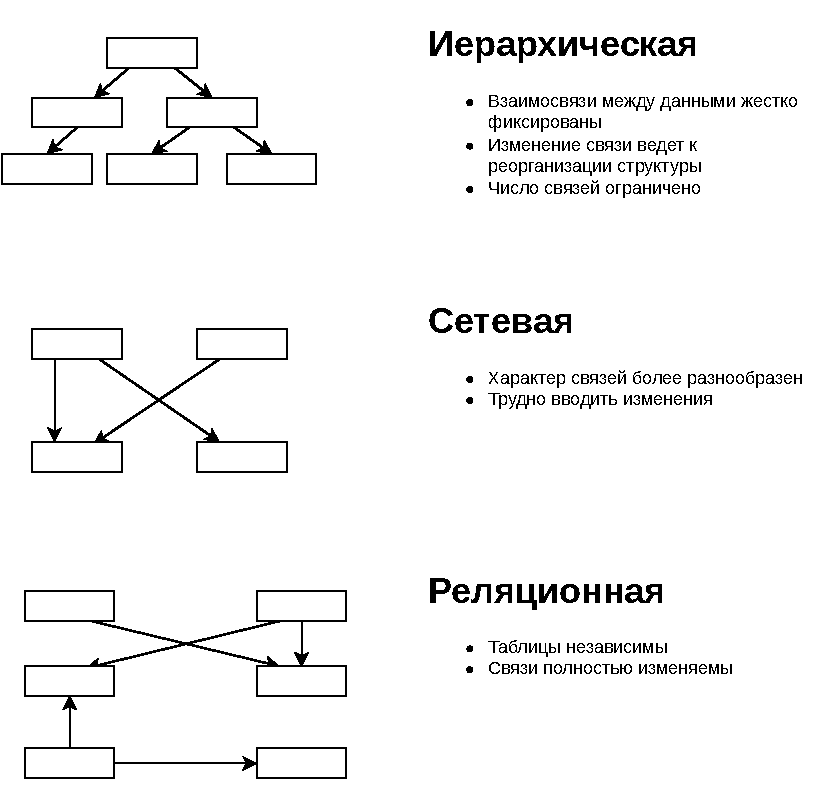
\includegraphics[width=0.9\linewidth]{assets/subd_classes.pdf}}
%	\caption{Классификация СУБД по модели данных}
%	\label{ris:subd-classes}
%\end{figure}
%
%\section{Вывод}
%
%В данном разделе была проанализирована поставленная задача и рассмотрены способы ее реализации. Также были рассмотрены разные типы СУБД. В качестве используемой в данной работе была выбрана реляционная СУБД PostgreSQL.